% This is LLNCS.DEM the demonstration file of
% the LaTeX macro package from Springer-Verlag
% for Lecture Notes in Computer Science,
% version 2.4 for LaTeX2e as of 16. April 2010
%
\documentclass{llncs}
%
\usepackage{makeidx}  % allows for indexgeneration
%\usepackage[LY1]{fontenc}
\usepackage[utf8]{inputenc}
\usepackage{ctable}
\usepackage{multirow}
\usepackage{hhline}
\usepackage{cite}
%\usepackage{algorithmicx}
\usepackage{algorithmic}
\usepackage{algorithm}
%\usepackage{algpseudocode}
\usepackage{xcolor}

%
\begin{document}
%
\frontmatter          % for the preliminaries
%
\pagestyle{headings}  % switches on printing of running heads
\addtocmark{Hamiltonian Mechanics} % additional mark in the TOC
\newcommand{\junk}[1]{}

%
%\tableofcontents
%
\mainmatter              % start of the contributions
%
\title{Improving genome assemblies using multi-platform sequence data}
%
\titlerunning{Improving genome assemblies}  % abbreviated title (for running head)
%                                     also used for the TOC unless
%                                     \toctitle is used
%
\author{Pınar Kavak\inst{1,2,*} \and Bekir Ergüner\inst{1}
Duran Üstek\inst{3} \and Bayram Yüksel\inst{4} \and Mahmut Şamil Sağıroğlu\inst{1} \and Tunga Güngör\inst{2} \and Can Alkan\inst{5,*}}
%

\authorrunning{Pınar Kavak et al.} % abbreviated author list (for running head)
%
%%%% list of authors for the TOC (use if author list has to be modified)
\tocauthor{Pınar Kavak, Bekir Ergüner, Duran Üstek, Bayram Yüksel, Mahmut Şamil Sağıroğlu, Tunga Güngör, Can Alkan}
%
\institute{Advanced Genomics and Bioinformatics Research Group (İGBAM), BİLGEM, The Scientific and Technological Research Council of Turkey (TÜBİTAK),\\
41470 Gebze, Kocaeli, Turkey\\
\email{pinar.kavak@tubitak.gov.tr}
\and
Department of Computer Engineering,
Boğaziçi University,\\ 
34342 Bebek, İstanbul, Turkey
\and
Department of Medical Genetics, 
İstanbul Medipol University,\\
34810 Beykoz, İstanbul, Turkey
\and
TÜBİTAK - MAM - GMBE (The Scientific and Technological Research Council of Turkey, Genetic Engineering and Biotechnology Institute),\\
41470 Gebze, Kocaeli, Turkey
\and
Department of Computer Engineering, 
Bilkent University,\\
06800 Bilkent, Ankara, Turkey\\
\email{calkan@cs.bilkent.edu.tr}
}


\maketitle              % typeset the title of the contribution

\begin{abstract}
Accurate \textit{de novo} assembly using short reads generated by next generation sequencing technologies is still an open problem. Although there are several assembly algorithms developed for data generated with different sequencing technologies, and some that can make use of hybrid data, the assemblies are still far from being perfect. There is still a need for computational approaches to improve draft assemblies.
Here we propose a new method to correct assembly mistakes when there are multiple types of data generated using different sequencing technologies that have different strengths and biases. We exploit the assembly of highly accurate short reads to correct the contigs obtained from less accurate  long reads.
We apply our method to Illumina, 454, and Ion Torrent data, and also compare our results with existing hybrid assemblers, Celera and Masurca.
\keywords{\textit{\textit{de novo}} assembly, assembly improvement, next generation multi-platform sequencing}
\end{abstract}
%
\section{Scientific Background}
Since the introduction of high throughput sequencing (HTS) technologies, traditional Sanger sequencing is being abandoned especially for large-scale sequencing projects.
Although cost effective for data production, HTS also imposes increased cost for data processing and computational burden. 
In addition, the data quality is in fact lower, with greater error rates, and short read lengths for most platforms. 
One of the main algorithmic problems in analyzing HTS data is the \textit{\textit{de novo}} assembly: i.e. ``stitching'' billions of short DNA strings into a collection of larger sequences, ideally the size of chromosomes. 
However, ``perfect'' assemblies with no gaps and no errors are still lacking due to many factors, including the short read and fragment (paired-end) lengths, sequencing errors in basepair level, and the complex and repetitive nature of most genomes. 
Some of these problems in \textit{de novo} assembly can be ameliorated through using data generated by different sequencing platforms, where each technology has ``strengths'' that may be used to fix biases introduced by others.

There are three kinds of assemblers mainly used to do genome assembly: i) greedy assemblers \cite{ssake:2007,sharcgs:2007,vcake:2007}, ii) overlap-layout-consensus (OLC) graph based assemblers \cite{celera:2000, sga:2012, hapsemblerDonmez:2011} and iii) de Bruijn graph based assemblers \cite{eulerPevzner:2008, abyssSimpson:2009, velvetZerbino:2008, spadesBankevich:2012, allpaths:2008}. Greedy assemblers follow a greedy approach such that: given one read or contig, at each step assembler adds one more read or contig with the largest overlap. The problem of greedy assemblers is that they can get stuck at local maxima. Therefore they are generally used for small genome assemblies. Since they also use more memory and are slower, it is not feasible to assemble large genomes with greedy assemblers.
OLC graph based assemblers work well when the long reads are available for assembly. They generate all-against-all pairwise alignments and build the graph by representing reads as nodes and overlaps between reads as edges. 
They obtain the consensus assembly by following a Hamiltonian path on the graph. 
Assemblers that are based on de Bruijn graphs are designed primarily for short reads. 
They use a k-mer graph approach instead of calculating all-against-all pairwise alignments. They build the graph by using k-mers as edges and the overlaps between k-mers as nodes. They follow an Eulerian path through the k-mer graph to find a consensus assembly.
Several assemblers use multiple read libraries \cite{cabogMiller:2008, masurcaZimin:2013, miraest, cerulian:2013} for better assembly construction. CABOG \cite{cabogMiller:2008} was initially designed for Sanger sequencing, and then it was revised to use 454 data, but it also accepts Illumina data to 
generate a hybrid assembly. Masurca \cite{masurcaZimin:2013} is able to assemble Illumina reads   together with longer 454 and Sanger reads. MIRAest \cite{miraest} can use Sanger, 454, Illumina, Ion Torrent and corrected PacBio data for hybrid assembly. It works on small genomes. Cerulean \cite{cerulian:2013} uses long PacBio reads and short Illumina reads to construct a hybrid assembly. It uses ABySS \cite{abyssSimpson:2009} assembler to generate \textit{assembly graphs} with paired end Illumina reads. Then, as input, it uses these \textit{assembly graphs} and also long PacBio read alignments to the assembled contigs.

Additionally, strategies to merge different assemblies using different data sources into a single coherent assembly are described in the literature (e.g. \cite{wang:2012}). Our method differs from that of \cite{wang:2012}, in data types. \cite{wang:2012} works on Illumina, 454 and ABI SOLID data, where we work on Illumina, 454 and Ion Torrent data. Also pre- and post-processing steps of the two methods differ. \cite{wang:2012} at first assembles 454, Illumina and SOLID data separately with different assemblers and then assembles the resulting contig collection again with another assembler.

In this work, we propose a method to improve draft assemblies (i.e. produced using a single data source, and/or single algorithm) by incorporating data generated by different HTS technologies, and by applying novel correction methods. To achieve better improvements, we exploit the advantages of both short but low-error-rate reads and long but erroneous reads. 
We show that correcting the contigs built by assembling long reads through mapping short and high quality read contigs produces the best results, compared to the assemblies generated by algorithms that use hybrid data all at once. With this study, we also have the opportunity to compare Ion Torrent and Roche/454 reads in terms of assembly performances.

\section{Materials and Methods}
\label{meth}
We  cloned a part of human chromosome 13 into a bacterial artificial chromosome (BAC), and 
sequenced it separately using Illumina, Roche/454, and Ion Torrent platforms (Table \ref{tab:dataprop}). 
We also obtained a ``gold standard'' reference assembly for this BAC  using GRCh37-guided assembly 
generated by  Mira~\cite{mira} using Roche/454 data, which we then corrected using the Illumina reads\cite{BACRef}. 
Since Roche/454 and Ion Torrent platforms have similar sequencing biases (i.e. problematic homopolymers), we separated this study into 
two different groups: Illumina \& 454 and Illumina \& Ion Torrent. We applied the same method on the two groups and 
evaluated them separately which gave us the opportunity to compare Roche/454 and Ion Torrent data. The flowchart of 
the pipeline is depicted in Figure \ref{fig:flowChart}.

\ctable[
      cap     = {},
      % 
      caption = {Properties of the data},
      % 
      label   = {tab:dataprop},
      doinside = \normalsize,
      width = 0.95\textwidth,
      %
      %
      pos = h!tb,
      star
]      {>{\raggedright\arraybackslash}X>{\raggedright\arraybackslash}X>{\raggedright\arraybackslash}
X>{\raggedright\arraybackslash}X>{\raggedright\arraybackslash}}
{
      \tnote[]{{\scriptsize \textbf{Technology}: The name of the sequencing technology used to produce the reads.
      \textbf{Length range}: Minimum and maximum lengths of the generated reads.
      \textbf{Mean length}: The mean length among all reads.
      \textbf{Mean base qual}: The average phred score sequence quality of all reads. Calculated by summing up all phred scores of the bases in a read and dividing it to sequence length of the read, over all reads.
      \textbf{Paired:} Represents whether the sequencing is performed as paired-end or single-end.}}
}
{ \FL
Technology & Length range & Mean length & Mean base qual (phred s.) & Paired \\ \ML
Illumina & 101bp \footnotesize{(all reads have equal length)} & 101bp & 38 & paired \\
\addlinespace[1mm]
Roche/454 & 40bp-1027bp & 650bp & 28 & single-end \\
\addlinespace[1mm]
Ion Torrent & 5bp-201bp & 127bp & 24 & single-end \\
\LL
}

\begin{figure*}[h!tbp]
\centerline{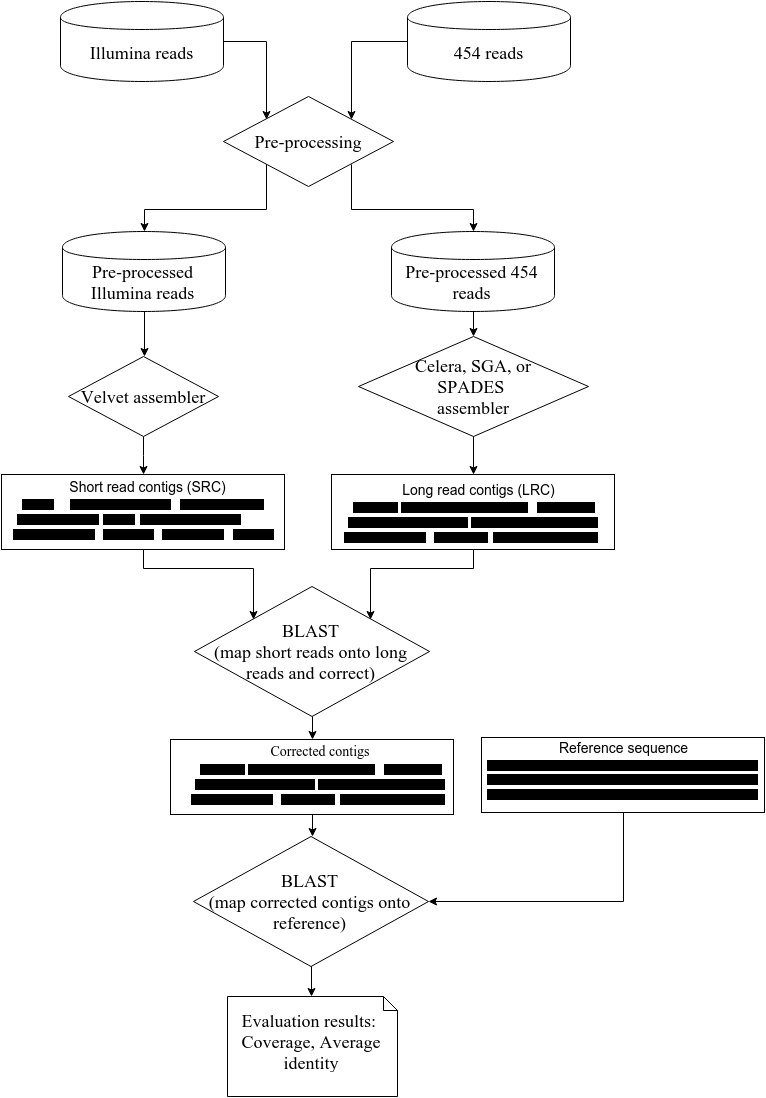
\includegraphics[width=12cm, height=18cm]{flowChart.png}}
\caption{Flow chart of the assembly improvement processes only for Illumina \& 454. Same is valid for Illumina \& Ion Torrent.}
\label{fig:flowChart}
\end{figure*}



\subsection{Pre-processing} 
\label{pre}
Pre-processing steps consist of the following: 
\begin{itemize}
\item First, we discard the reads that have low average quality value (phred score 17, i.e. $\geq$2\% error rate). 
\item Then, we remove the reads with high N-density (with $>$10\% of the read consisting of Ns) from consideration. Ns would destroy the assembly contiguity. 
\item Third, we trim the groups of bases at the beginning and/or at the end of the read that seem to be non-uniform according to sequence base content (A,T,G,C) (See Figure \ref{fig:nonuniformATGC}). These regions would cause erroneous structures in the assembly.
\item Finally, we apply the pre-processing operations of each assembler we used.
\end{itemize}


\begin{figure*}[h!tbp]
\centerline{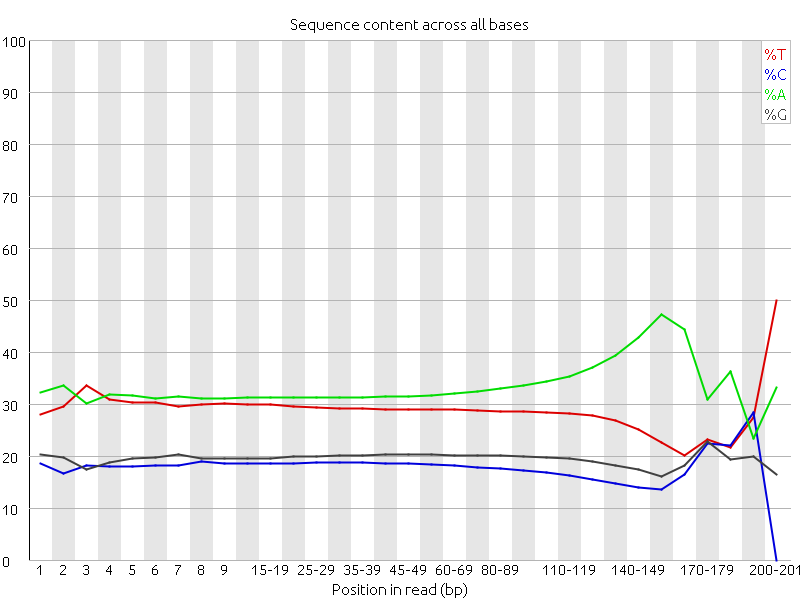
\includegraphics[width=12cm, height=8.2cm]{ionTorrentFastqc.png}}
\caption{Non-uniform A,T,G,C regions of Ion Torrent reads. First 8 bases and the bases after the 130$^{th}$ base are trimmed in pre-processing.}
\label{fig:nonuniformATGC}
\end{figure*}


\subsection{Assembly}
\label{ass} 
After the pre-processing step, we used several assembly tools suitable to assemble different types of data: We used Velvet~\cite{velvetZerbino:2008}, a de Bruijn graph based assembler that is designed to assemble short reads for assembling the Illumina reads. Considering the trimmed beginning and/or end parts of 101bp long paired-end reads from Illumina, and after testing kmers 21 and 31, we decided to use k=51 for short read assembly. We ran Velvet with {\tt shortPaired} mode with insert size 400bp, expected coverage 80, coverage cutoff 2, and minimum contig length 100. N50 value of the resulting short read contigs was 8,865 bp. We used two different OLC assemblers: Celera~\cite{celera:2000} and SGA~\cite{sga:2012} to assemble the long read data sets (Roche/454 and Ion Torrent) separately. We ran Celera assembler in {\tt unmated} mode and with default parameters to assemble 454 and Ion Torrent reads. N50 value of the assembly obtained with 454 and Ion Torrent reads with Celera was 1,308 bp and 1,284 bp, respectively. We also used SGA assembler in unmated mode for the same data sets. We obtained N50 values of 505 bp and 117 bp for Roche/454 and Ion Torrent data, respectively. In addition, we also used a de Bruijn graph based assembler, SPAdes~\cite{spadesBankevich:2012}, to assemble the long read data. Again, we applied default parameters. 
N50 values of the assemblies obtained with 454 and Ion Torrent reads with SPAdes were 212 bp and 259 bp, respectively.

We mapped all draft assemblies to the E. coli reference sequence using BLAST~\cite{blast}'s MegaBLAST ~\cite{megablast} task to identify and discard E. coli contamination due to the cloning process. We discarded any contig that mapped to the E. coli reference sequence with sequence identity $\geq$95\%. Finally, we obtained one short read, and three long read assemblies without contamination.

\subsection{Correction} 
\label{correc}
In the correction phase, we wanted to exploit the accuracy of the short read contigs (SRC) and the coverage of the long read contigs (LRC) to obtain a better assembly. 
Hence, we mapped all SRCs onto all LRCs of each group and corrected the LRCs according to the mapping results.
First, we used BLAST~\cite{blast}'s MegaBLAST \cite{megablast} mapping task to map the SRC onto the LRC.
We then used an in-house C++ program to process the MegaBLAST mapping results. 
Since MegaBLAST may report multiple mapping locations due to repeats, we only accepted the ``best'' mapping locations. 
Reasoning from the fact that short reads show less sequencing errors, we preferred the sequence reported by the SRC over the LRC when there is a disagreement between the pair. 
By doing this, we patched the ``less fragmented'' long read assemblies. 
If there is an overlap between different SRC mappings at the same region on the LRC, the latter overwrites the first. 
Figure \ref{fig:correction} shows a visual representation of the strategy on correcting the LRCs. 

Briefly, we describe our strategy in the following steps: 
\begin{itemize}
\item If there is a mapping between a SRC and a LRC, and if the mapping does not start at the beginning of the LRC, add the unmapped prefix of the LRC. 
\item Next, if the mapping does not start at the beginning of the SRC (very rare situation), add the unmapped prefix of the SRC with lowercase (i.e. low confidence) letters. 
\item Over the mapping region between SRC and LRC, pick the SRC values. 
\item If the mapping does not end at the end of the SRC (rare), add the unmapped suffix of the SRC, again with lowercase letters. One may argue that it might disturb the continuity of the resulting contig, however, we observe such mapping properties very rarely. The reason for using lowercase letters is to keep track of the information that there is a disagreement between the SRC and LRC on these sections, so the basepair quality will be lower than other sections of the assembly. 
\item Finally, add the unmapped suffix of the LRC and obtain the corrected contig.
\end{itemize}
We repeated this process to correct each of the three long read assembly contig sets. We applied our correction strategy on each data set multiple times until there is no improvement in the
{\it Coverage} and  {\it Average Identity} metrics. 


\begin{figure*}[h!tbp]
\centerline{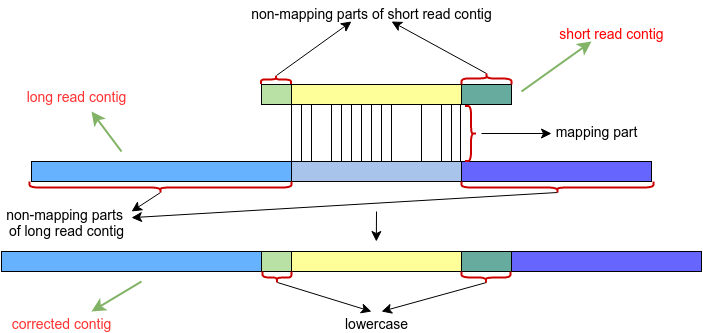
\includegraphics[width=12cm, height=5cm]{BACAlgorithm.png}}
\caption{Correction method: Correct the long read contig according to the mapping information of the short read contig.}
\label{fig:correction}
\end{figure*}

\subsection{Evaluation}
\label{eval}

To evaluate and compare the resulting and corrected assemblies all-against-all, we mapped all of the assembly candidates, including primary assemblies and also final corrected assemblies to the ``gold standard'' BAC assembly. According to the alignment results, we calculated various statistics such as the number of mapped contigs, how many bases on the reference sequence were covered, how many gaps exist on the reference sequence, and the total gap length. We calculated metrics such as ``Coverage'' and ``Average Identity'' and compared the resulting assemblies with these metrics. 

To calculate these statistics, we kept an array of arr{\_}reference[0,0,0,...0], where 
\\length(arr{\_}reference)= length(reference). 
We updated the contents of arr{\_}reference according to the alignments. 
If there is a match at a location, we assigned the corresponding position in the array to ``1'', if there is a mismatch at a location, 
we set it as ``-1'', and if that location is not included in any alignment, we left it as ``0'' 
(which means a gap). We assumed deletions in the contig (query) as mismatches. 
We also calculated the number of insertions in the contig. 
Scanning the array and summing up the number of ``1''s (matches), ``-1''s (mismatches), ``0''s (gaps) and ``insertionInQuery'', we obtained the number of matches, mismatches, gaps, and insertions in contig. 
Using these numbers, we calculated the Coverage (Equation~\ref{eqn:coverage}) and Average Identity values (Algorithm~\ref{alg:avgident}).

We also used two hybrid assemblers, Celera-CABOG~\cite{cabogMiller:2008} and Masurca \cite{masurcaZimin:2013}, with Illumina \& 454 and Illumina \& Ion Torrent. These hybrid assemblers load all reads as input and assemble them with a hybrid method. We assembled the two data sets with these hybrid assemblers to compare our correction method with the results of them. 


\begin{equation}
\label{eqn:coverage}
\textnormal{Coverage} = \left(\frac{\textnormal{\#{ }of{ }covered{ }bases}}{\textnormal{length of the reference}}\right)
\end{equation}


\junk{
  \begin{equation}
    
    \textcolor{blue}{do\{}\\

\qquad{} alignmentLength = matches + mismatches +  insertionInContig\\

\qquad{} \textnormal{identity} = \left(\frac{\textnormal{matches}}{\textnormal{alignmentLength}}\right)\\

\qquad{} avgIdentity = \textnormal{avgIdentity} + \textnormal{identity} \times \textnormal{contigLength}\\

\intertext{\textcolor{blue}{\}while(\textnormal{no contigs left})}}\\

avgIdentity =\left(\frac{\textnormal{avgIdentity}}{\sum_{i=1}^{contigNum}{contigLength}_i}\right) \qquad{}\qquad{}\qquad{}\qquad{}\qquad{}\qquad{}\qquad{}\qquad{}\qquad{}
%avgIdentity =\left(\frac{\textnormal{avgIdentity}}{\textnormal{sumOfContigLengths}}\right)
\end{equation}
}

\begin{algorithm}
\caption{Average identity} % give an algorithm name
\label{alg:avgident}
\begin{algorithmic}
  \WHILE {\mbox{no contigs left}}
  \STATE {alignmentLength $\gets$ matches + mismatches +  insertionInContig}\\
  \STATE {\textnormal{identity} $\gets$ $\left(\frac{\textnormal{matches}}{\textnormal{alignmentLength}}\right)$}\\
  \STATE {~~~avgIdentity $\gets$ \textnormal{avgIdentity} + \textnormal{identity} \times \textnormal{contigLength}}
  \ENDWHILE
  \STATE{avgIdentity $\gets$ $\left(\frac{\textnormal{avgIdentity}}{\sum_{i=1}^{contigNum}{contigLength}_i}\right)$} 
\end{algorithmic}
\end{algorithm}



\ctable[star
	    center
      cap     = {},
      % 
      caption = {Results of assembly correction method on BAC data.},
      % 
      label   = {tab:resultsTable},
      doinside = \tiny,
      width = 1\textwidth,
      %maxwidth=19cm,
      %
      %
       pos = h!tbp      
       ]
       {c>{\raggedright\arraybackslash}X>{\raggedright\arraybackslash}X>{\raggedright\arraybackslash}
         X>{\raggedright\arraybackslash}X>{\raggedright\arraybackslash}X>{\raggedright\arraybackslash}
         X>{\raggedright\arraybackslash}X>{\raggedright\arraybackslash}}
       {         
        \tnote[]{{\tiny Name: the name of the data group that constitutes the assembly; \# of Contigs: the number of contigs that belong to the resulting assembly; \# of Mapped Contigs: the number of contigs that successfully mapped onto the reference sequence; \# of Covered bases: the number of bases on the reference sequence that are covered by the assembly; Coverage: percentage of covered reference; Avg. identity: percentage of the correctly predicted reference bases; \# of Gaps: the number of gaps that cannot be covered on the reference genome; Size of Gaps: total number of bases on the gaps.}}
         \tnote[*]{{\tiny ``2'' represents the results of the second cycle of correction, ``3'' represents the third cycle.}}
         \tnote[\#]{{\tiny A mistake is noticed on Ill-454 Celera data and the results are corrected after being published in the proceedings of CIBB2015.}}
       }
       {
         \FL
         Name & Length & \# of Contigs & \# of Mapped Contigs & \# of Covered bases & Coverage & Avg. Identity & \# of Gaps & Size of Gaps\ML
		 \textbf{\textit{Reference}} & \textit{176.843} & & & & & & & \ML
		 \addlinespace
		 \textbf{Velvet} & & & & & & & \NN
         Ill. Velvet & 197,040 & 455 & 437 & 175,172 & 0.99055 & 0.97523 & 39 & 1,671 \ML
         \textbf{Celera} & & & & & & & \NN       
         454 Celera & 908,008 & 735 & 735 & 172,563 & 0.97580 & 0.92599 & 18 & 4,280 \NN
         Ion Celera & 39,347 & 27 & 27 & 47,638 & 0.26938 & 0.96932 & 47 & 129,205 \ML
         \addlinespace
         \textbf{Corrected Celera}\tmark[\#] & & & & & & & \NN
         Ill-454 Celera & 371,065 & 250 & 250 & 176,071 & 0.995635 & 0.944558 & 5 & 772 \NN
         Ill-454 Celera^2\tmark[*] & 365,802 & 245 & 245 & 176,343 & 0.9971 & 0.9455 & 4 & 500 \NN
         Ill-Ion Celera & 93,909 & 30 & 28 & 81,819 & 0.46267 & 0.96327 & 36 & 95,024 \NN
         Ill-Ion Celera^2 & 145,262 & 30 & 28 & 91,962 & 0.52002 & 0.97412 & 33 & 84,881 \NN
         Ill-Ion Celera^3 & 216,167 & 30 & 28 & 99,645 & 0.56347 & 0.98066 & 34 & 77,198 \ML
         \textbf{SGA} & & & & & & & \NN
         454 SGA & 62,909,254 & 108,095 & 101,514 & 176,546 & 0.99832 & 0.97439 & 1 & 297 \NN
         Ion SGA & 842,997 & 6,417 & 6,122 & 153,092 & 0.86569 & 0.99124 & 197 & 23.751 \ML	
         \addlinespace
         \textbf{Corrected SGA} & & & & & & & \NN
         Ill-454 SGA & 295,009 & 335 & 335 & 176,757 & 0.99951 & 0.96823 & 5 & 86 \NN
%         Ill-454 SGA^2 & 279,034 & 305 & 305 & 176,757 & 0.99951 & 0.96769 & 5 & 86 \NN
         Ill-Ion SGA & 197,509 & 291 & 291 & 175,052 & 0.98987 & 0.97501 & 45 & 1,791 \NN
         Ill-Ion SGA^2 & 203,064 & 291 & 291 & 175,676 & 0.99340 & 0.97413 & 34 & 1,167 \ML
%         Ill-Ion SGA^3 & 204,524 & 291 & 291 & 175,677 & 0.99341 & 0.97405 & 34 & 1,166 \ML
         \textbf{SPADES} & & & & & & & \NN
         454 SPADES & 12,307,761 & 49,824 & 49,691 & 176,843 & 1.0 & 0.98053 & 0 & 0 \NN
         Ion SPADES & 176,561 & 110 & 107 & 167,890 & 0.94937 & 0.92909 & 9 & 8,953 \ML	
         \addlinespace
         \textbf{Corrected SPADES} & & & & & & & \NN
         Ill-454 SPADES & 290,702 & 298 & 298 & 176,454 & 0.99780 & 0.96538 & 5 & 389 \NN
%         Ill-454 SPADES^2 & 290,917 & 297 & 297 & 176,454 & 0.99780 & 0.96530 & 5 & 389 \NN
%         Ill-454 SPADES^3 & 291.653 & 297 & 297 & 176.454 & 0.99780 & 0.96527 & 5 & 389 \NN
         Ill-Ion SPADES & 198,665 & 52 & 52 & 171,977 & 0.97248 & 0.94215 & 4 & 4,866 \NN
         Ill-Ion SPADES^2 & 200,307 & 52 & 52 & 172,101 & 0.97319 & 0.94230 & 2 & 4,742 \ML
         \textbf{Masurca} & & & & & & & \NN
         Ill-454 Masurca & 380 & 1 & 0 & 0 & 0 & 0 & 0 & 0 \NN
         Ill-Ion Masurca & 2,640 & 8 & 8 & 1,952 & 0.01104 & 0.98223 & 9 & 174,891 \ML
 		\textbf{Celera-CABOG} & & & & & & & \NN
         Ill-454 Celera & 1,101,716 & 891 & 891 & 174,330 & 0.98579 & 0.92452 & 12 & 2,513 \NN
         Ill-Ion Celera & 0 & 0 & 0 & 0 & 0.0 & 0.0 & 0 & 0.0 \NN
         \LL
       }
\vspace*{-0.3cm}

\ctable[star
	    center
      cap     = {},
      % 
      caption = {Results with combination of 3 data types},
      % 
      label   = {tab:resultsTable3data},
      doinside = \tiny,
      width = 1\textwidth,
      %maxwidth=19cm,
      %
      %
       pos = h!tbp      
       ]
       {c>{\raggedright\arraybackslash}X>{\raggedright\arraybackslash}X>{\raggedright\arraybackslash}
         X>{\raggedright\arraybackslash}X>{\raggedright\arraybackslash}X>{\raggedright\arraybackslash}
         X>{\raggedright\arraybackslash}X>{\raggedright\arraybackslash}}
       {         
        \tnote[]{{\tiny Name: the name of the data group that constitutes the assembly; \# of Contigs: the number of contigs that belong to the resulting assembly; \# of Mapped Contigs: the number of contigs that successfully mapped onto the reference sequence; \# of Covered bases: the number of bases on the reference sequence that are covered by the assembly; Coverage: percentage of covered reference; Avg. identity: percentage of the correctly predicted reference bases; \# of Gaps: the number of gaps that cannot be covered on the reference genome; Size of Gaps: total number of bases on the gaps.}}
        \tnote[*]{{\tiny ``2'' represents the results of the second cycle of correction, ``3'' represents the third cycle.}}
       }
       {
         \FL
         Name & Length & \# of Contigs & \# of Mapped Contigs & \# of Covered bases & Coverage & Avg. Identity & \# of Gaps & Size of Gaps\ML
		 \textbf{\textit{Reference}} & \textit{176.843} & & & & & & & \ML
		 \addlinespace
		 \textbf{Corrected Ion Celera} & & & & & & & \NN
         454-Ion Celera & 500,251 & 27 & 27 & 149,021 & 0.84267 & 0.94515 & 63 & 27,822 \NN
         Ill-``454-Ion Celera'' & 570,865 & 27 & 27 & 170,348 & 0.96327 & 0.95503 & 16 & 6,495 \NN
         Ill-``454-Ion Celera''^2\tmark[*] & 575,726 & 27 & 27 & 172,516 & 0.97553 & 0.95541 & 12 & 4,327 \NN
         Ill-``454-Ion Celera''^3 & 578,727 & 27 & 27 & 174,535 & 0.98694 & 0.95555 & 10 & 2,308 \ML
		\textbf{Corrected Ion SPADES} & & & & & & & \NN
         454-Ion SPADES & 11,224,602 & 60 & 60 & 176,540 & 0.99828 & 0.97334 & 6 & 303 \NN
         Ill-``454-Ion SPADES'' & 9,543,712 & 45 & 45 & 176,712 & 0.99925 & 0.97347 & 1 & 131 \ML
         \textbf{Corrected Ion SGA} & & & & & & & \NN
         ``Ill-454''-Ion SGA & 281,155 & 212 & 212 & 176,769 & 0.99958 & 0.96562 & 4 & 74 \ML
%         Ill-``Corr-454-Ion SGA'' & 280,344 & 207 & 207 & 176,573 & 0.99847 & 0.96557 & 5 & 270 \ML              
         \textbf{Masurca(all)} & & & & & & & \NN
         Ill-454-Ion Masurca & 3,398 & 7 & 5 & 1,477 & 0.00835 & 0.99363 & 5 & 175366 \ML
 		\textbf{Celera-CABOG(all)} & & & & & & & \NN
         Ill-454-Ion Celera & 575,642 & 485 & 485 & 164,621 & 0.93088 & 0.94664 & 39 & 12,222 \NN
         \LL
       }
\vspace*{-0.3cm}

\section{Results}
\label{bacResultsConc}

We present the results in Table \ref{tab:resultsTable}, and interpret them in different point of views. 

\subsection{454 vs. Ion Torrent}
\label{454Ion}
Ion Torrent reads are shorter than 454 reads and they have less mean base quality (Table \ref{tab:dataprop}). So, we did not expect to have better assembly with Ion Torrent reads than 454 reads. The results in Table \ref{tab:resultsTable} agree with our expectations.
In Table \ref{tab:resultsTable}, we see that the assembly of 454 reads performs better on evaluation metrics than Ion Torrent with all kind of assemblers. The assembly of Ion Torrent reads with Celera assembler has very low coverage value: 26.94\%. The reason for the low coverage might be because Celera assembler is not designed for Ion Torrent read type (shorter reads with lower quality). Even 454 and Ion Torrent reads have similar error types at the homopolymer regions. SGA assembly with Ion Torrent reads performs better on Coverage (86.57\%) but it cannot reach to the Coverage of SGA assembly with 454 reads (99.83\%). The assembly of Ion Torrent reads has the highest coverage with SPAdes assembler (94.94\%). Correction of the Ion Torrent contigs improves the assembly quality but even after correction phase Ion Torrent corrected assembly cannot reach the results of 454 corrected assembly. 

\subsection{Assemblers}
\label{res_ass}
Table \ref{tab:resultsTable} shows that the assembly obtained by Velvet with only short Illumina reads showed good coverage  (99.05\%) and average identity rates (97.52\%). The number of contigs obtained with Velvet assembly is 455, of which 437 map to the reference. There are 39 gaps and the total size of the gaps is 1,671 bp. Our aim was to increase the coverage, improve the average identity, decrease the number of contigs and gaps, and shrink the lengths of the gaps.

Since we observed that 454 reads resulted better assembly than Ion Torrent reads as stated in Section \ref{454Ion}, we compared different assemblers using 454 contigs. The assembly of Celera with the 454 long reads has 97.58\% coverage and 92.59\% average identity, which are lower than Illumina-Velvet values. Number of contigs (735) is reasonable but number of gaps and total gap length are high (18 and 4,280 bp, respectively). 
SGA assembly using 454 reads has very high coverage (99.83\%) and identity (97.43\%). It has just one gap with size 297 bp, but the number of contigs is also very high (101,514), which is an unwelcome situation. SPAdes-454 assembly also had a large number of contigs (49,824) which completely cover the reference sequence with 98.05\% average identity. SPAdes assembly resulted in lower number of contigs and had higher coverage and average identity than SGA. 
If we evaluate the results according to the number of contigs, Celera-454 results seem more reasonable than SGA or SPAdes results, since it returned a reasonable number of contigs even with low coverage and average identity.

\subsection{Correction}
\label{res_corr}
We observed that the correction method improved both 454 and Ion Torrent based assemblies generated with all assemblers we tested (Table \ref{tab:resultsTable}). In the remainder of the paper, we only mention the 454-based assemblies for simplicity.

When we applied our correction method on Celera-454 assembly using the Velvet-Illumina assembly, we achieved better coverage and average identity rates: the coverage of 454 assembly increases up to 99.56\% and the average identity rate increases up to 94.45\% on the first correction cycle. The second correction cycle increases the coverage and average identity rates to 99.71\% and 94.55\%, respectively, and the correction converges. The number of contigs decrease to 245 from 735, and the number of gaps decrease down to 4 (500 bp) from 18 (4,280 bp). Since the third correction cycle does not give better results it is not shown in Table \ref{tab:resultsTable}.

Our correction method increased the coverage of SGA-454 assembly up to 99.99\% from 99.82\% but with less average identity and with more gaps although the total length of the gaps is decreased. Correction using the short read assembly decreased the number of contigs down to a reasonable number (335). Corrected SGA assembly has the largest coverage rate among all, and also with more identity than Velvet-Illumina assembly.

The number of contigs in SPAdes assembly also decreased to 298 from 49,691 using our correction method. With the decrease in number of contigs, the coverage also decreased (99.78\%) as well as the average identity (96.53\%). The number of gaps increased to 5 from 0 with a total size of 389.

In summary, we obtained substantial assembly correction in draft assemblies by using advantages of different technologies.

\subsection{Hybrid Assemblers}
\label{hyb}

We also compared the results of two hybrid assemblers on our multiple type of data. We ran Masurca and Celera-CABOG with default parameters given two groups of hybrid data as input: Illumina \& 454 and Illumina \& Ion Torrent. Hybrid assemblers Masurca and CABOG did not show good assembly rates.
We obtained zero coverage with 454 and Illumina reads using Masurca. The only contig left after the contamination removal did not map to the reference sequence. We also observed very low coverage (1.10\%) with 98.22\% average identity  with Ion Torrent \& Illumina reads. Therefore, we conclude that Masurca did not work very well in our case with our data types. 

Similarly, we obtained zero coverage with Ion Torrent \& Illumina using CABOG. All of the resulting contigs obtained from the assembly were removed as contamination. However, CABOG performed substantially better with
Illumina \& 454, and generated assembly with 98.58\% coverage and 92.45\% average identity.
The assembly composed of 891 contigs and 12 gaps with total gap length of 2,513 bp. Still, 
the performance of CABOG was not better than the corrected assembly results described above.

\subsection{All Data Together}
\label{3data}
We combined all 3 data types in order to see if we have better coverage or accuracy on the results. The results are presented in Table \ref{tab:resultsTable3data}. Since our method works as correcting one data type's contigs with the other data type's contigs, we needed to combine three types of contigs sequentially. As mentioned in Section \ref{correc} our method accepts that the corrector data is more accurate than the corrected data. If there is a map between the two, it replaces the values of the corrected data with the values of the corrector data. For that reason, while working with 3 data combination, we decided to use Velvet-Illumina contigs which are built by the highest accurate reads as the last corrector. On Table \ref{tab:resultsTable3data}, it is seen that Celera-454 contigs increase the coverage rate of Celera-Ion Torrent contigs (from 26.93\% to 84.26\%) although decreasing the average identity rate from 96.93\% to 94.51\%. Correcting the resulting contigs with Velvet-Illumina contigs increases the coverage (96.32\%) and average identity rates (95.50\%) even higher. The coverage and average identity rates are improved on the second and third cycles too. Correcting Ion SPADES, with 454 SPADES gives higher coverage (99.82\%) and average identity (97.33\%) rates than correcting them with only Velvet Illumina contigs (97.24\% and 94.21\% respectively). After using Velvet Illumina contigs for the last correction, the results are improved approximately by 0.1\% and 0.01\% respectively. Correcting Ion SGA contigs with 454 SGA contigs was not possible because of memory limitations of BLAST mapping with such huge data. Instead, we used corrected version of ``454 SGA contigs with Illumina Velvet contigs'' to correct the Ion SGA contigs. The coverage is higher than both Ill-Ion SGA and Ill-454 SGA, average identity is lower than Ill-454 SGA. 

We also ran the hybrid assemblers Masurca and CABOG with default parameters with the combination of three data. Masurca resulted in very low coverage 0.8\% as it did before with the dual combinations. CABOG resulted in lower coverage and higher average identity compared to Ill-454 combination and higher in both compared to Ill-Ion Torrent combination. Hybrid assembler still did not result in as high coverage and average identity as obtained with the correction method.

We note that exploiting all the data gives us more accurate results especially when we are using a diverse data which has different strengths and weaknesses. However, one must be careful about the weaknesses and strengths of the data and where and in which order to use each them.
\section{Conclusion}
\label{concl}
In this paper, we presented a novel method to improve draft assemblies by correcting high contiguity assemblies using the relatively more fragmented contigs obtained using high quality short reads. Assembling short and long reads separately using both de Bruijn and OLC graph based assemblers according to data types and then using correction methods gives better results than using only hybrid assemblers. Using three data types together for correction or as the input of te hybrid assemblers rather than using only two of them gives more accurate results.

However, the need to develop new methods that exploit different data properties of different HTS technologies, such as short/long reads or high/low quality of reads, remains. In this manner, as future work, our correction algorithm can be improved by exploiting the paired end information of the short, high quality reads after the correction phase to close the gaps between corrected contigs.

\paragraph{Funding.}

The project was supported by the Republic of Turkey Ministry of Development Infrastructure Grant (no: 2011K120020), BİLGEM TÜBİTAK (The Scientific and Technological Research Council of Turkey) grant (no: T439000), and a TÜBİTAK grant to Can Alkan(112E135).\\

%\newpage
%
% ---- Bibliography ----
%
\begin{thebibliography}{}
%

\bibitem{ssake:2007} R.L.Warren, G.G.Sutton, S.J.M.Jones, R.A.Holt: Assembling millions of short DNA sequences using SSAKE, Bioinformatics, 23(4):500-501 (2007)
\bibitem{sharcgs:2007} J.C.Dohm, C.Lottaz, T.Borodina, H.Himmelbauer: SHARCGS, a fast and highly accurate short-read assembly algorithm for \textit{de novo} genomic sequencing, Genome Research, 17(11):1697-1706 (2007)
\bibitem{vcake:2007} W.R.Jeck, J.A.Reinhardt, D.A.Baltrus, M.T.Hickenbotham, V.Magrini, E.R.Mardis, J.L.Dangl, C.D.Jones: Extending assembly of short DNA sequences to handle error, Bioinformatics, 23(21):2942-2944 (2007)
\bibitem{hapsemblerDonmez:2011} N.Donmez, M.Brudno: Hapsembler: An Assembler for Highly Polymorphic Genomes, Proceedings of the 15th Annual International Conference on Research in Computational Molecular Biology, pages:38-52 (2008)
\bibitem{celera:2000} E.W.Myers, G.G.Sutton, A.L.Delcher, I.M.Dew, D.P.Fasulo, M.J.Flanigan, S.A.Kravitz, C.M.Mobarry \textit{et~al}: A Whole-Genome Assembly of Drosophila, Science, {287(no:5461)}:2196-2204, doi:10.1126/science.287.5461.2196 (2000)
\bibitem{sga:2012} J.Simpson R.Durbin: Efficient \textit{de novo} Assembly of Large Genomes Using Compressed Data Structures, Genome Research, {22}:549-556, doi:10.1101/gr.126953.111 (2012)
\bibitem{velvetZerbino:2008} D.R.Zerbino, E.Birney: Velvet: Algorithms for \textit{de novo} Short Read Assembly Using de Bruijn Graphs, Genome Research, {18(5)}:821-829, doi: 10.1101/gr.074492.107 (2000)
\bibitem{spadesBankevich:2012} A.Bankevich, S.Nurk, D.Antipov, A.A. Gurevich, M.Dvorkin, A.S.Kulikov, V.M.Lesin, S.I.Nikolenko {\it et~al}: SPAdes: A New Genome Assembly Algorithm and Its Applications to Single-Cell Sequencing, Journal of Computational Biology, {19(5)}:455-477, doi:10.1089/cmb.2012.0021 (2012)
\bibitem{allpaths:2008} J.Butler, I.MacCallum, M.Kleber, I.A.Shlyakhter, M.K.Belmonte, E.S.Lander, C.Nusbaum, D.B.Jaffe: ALLPATHS: \textit{De novo} Assembly of Whole-Genome Shotgun Microreads, Genome Research, {18(5)}:810-820, doi:10.1101/gr.7337908 (2008)
\bibitem{abyssSimpson:2009} J.T.Simpson, K.Wong, S.D.Jackman, J.E.Schein, S.J.M.Jones, İ.Birol ABySS: A parallel assembler for short read sequence data, Genome Research, 19(6):1117-1123 (2009)
\bibitem{eulerPevzner:2008} M.J.Chaisson, D.Brinza, P.A.Pevzner: \textit{De novo} fragment assembly with short mate-paired reads: Does the read length matter?, Genome Research, 19(2):336-346 (2008)
\bibitem{cabogMiller:2008} J.R.Miller, A.L.Delcher, S.Koren, E.Venter, B.P.Walenz, A.Brownley, J.Johnson, K.Li, C.Mobarry, G.Sutton: Aggressive Assembly of Pyrosequencing Reads with Mates, Bioinformatics, {24(24)}:2818-2824, doi:10.1093/bioinformatics/btn548 (2008)
\bibitem{masurcaZimin:2013} A.Zimin, G.Mar\c{c}ais, D.Puiu, M.Roberts, S.L.Salzberg, J.A.Yorke: The MaSuRCA Genome Assembler, Bioinformatics, {29(21)}:2669-2677, doi:10.1093/bioinformatics/btt476 (2013)
\bibitem{mira} B.Chevreux, T.Wetter, S.Suhai:  Genome Sequence Assembly Using Trace Signals and Additional Sequence Information, Computer Science and Biology:Proceedings of the German Conference on Bioinformatics (GCB), {99}:45-56 (1999)
\bibitem{miraest} B.Chevreux, T.Pfisterer, B.Drescher, AJ.Driesel, WE.Müller, T.Wetter, S.Suhai: Using the miraEST assembler for reliable and automated mRNA transcript assembly and SNP detection in sequenced ESTs, Genome Research, 14(6), 1147-1159 (2004)
\bibitem{cerulian:2013} V.Deshpande, E.D.Fung, S.Pham, V.Bafna: Cerulean: A hybrid assembly using high throughput short and long reads, arXiv:1307.7933 [q-bio.QM] (2013)
\bibitem{BACRef} B.Ergüner, D.Ustek, MŞ. Sağıroğlu: Performance Comparison of Next Generation Sequencing Platforms, Poster presented at: 37th International Conference of the IEEE Engineering in Medicine and Biology Society (2015)
\bibitem{wang:2012} Y.Wang, Y.Yao, P.Bohu, H.Pei, L.Yixue, S.Zhifeng, X.Xiaogang, L.Xuan: Optimizing Hybrid Assembly of Next-Generation Sequence Data from Enterococcus Faecium: a Microbe with Highly Divergent Genome, BMC Systems Biology, {6(Suppl 3)}:S21, doi:10.1186/1752-0509-6-S3-S21 (2012)
\bibitem{blast} S.Altschul, W.Gish, W.Miller, E.Myers, D.J.Lipman: Basic Local Alignment Search Tool, Journal of Molecular Biology, {215(3)}:403-410 (1990)
\bibitem{megablast} Z. Zhang, S. Schwartz, L. Wagner, W. Miller: A greedy algorithm for aligning {DNA} sequences. J Comput Biol, 7(12):203-214 (2000)



\end{thebibliography}
\clearpage
\addtocmark[2]{Author Index} % additional numbered TOC entry
\renewcommand{\indexname}{Author Index}
\printindex
\clearpage
\addtocmark[2]{Subject Index} % additional numbered TOC entry
\markboth{Subject Index}{Subject Index}
\renewcommand{\indexname}{Subject Index}
%\input{subjidx.ind}
\end{document}
